\section{Epipolar Geometry and Chaining}
\label{egc}
In this section we are going to describe the first part of the Structure from Motion algorithm, which is to exploit prior knowledge about the scene. This is done by finding corresponding image points in multiple views and compute their epipolar geometry which is expressed algebraically by the fundamental matrix which can be decomposed to obtain the required projection matrices.

\subsection{Dataset}
The data we were required to use consists of two individual datasets. The first one contains 49 frames, each one of them depicting a house from a different angle. The second contains 16 frames, each one of them depicting a teddy-bear from a different view. In each frame, there is a slight movement of the target object with respect to the previous frames.

\subsection{Implementation}
An important step of the algorithm is to identify local features in each image which are consistent in most of the frames. For this purpose we used the  Scale-Invariant Feature Transform (SIFT) (vl\_ sift function in vlFeat library) algorithm to detect points of interest in each frame. In order to restrict the search process of the SIFT detector an active contour based segmentation was used. By applying this technique we were able to segment the frames into background and foreground regions, allowing us to focus only on the points that exist on the object of interest as presented in figure~\ref{fig:houseBackground}.

\begin{figure}[ht!]
  \centering
    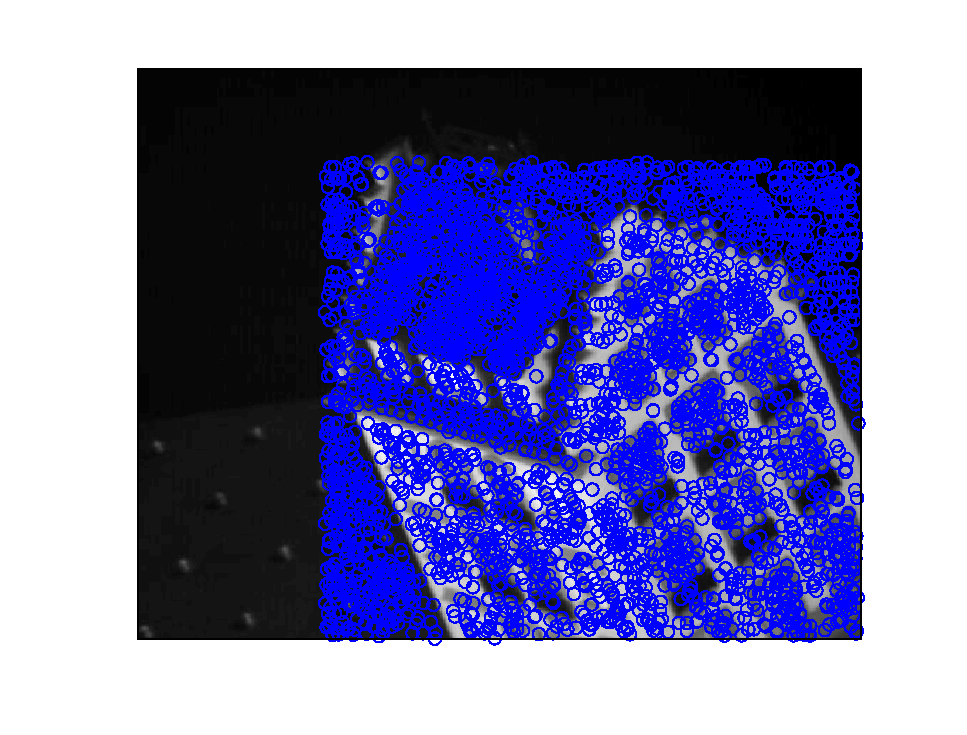
\includegraphics[width=0.49\textwidth]{figures/houseBackground.eps}
    \caption{Feature points extracted by the SIFT detector found on the object of interest}
    \label{fig:houseBackground}
\end{figure}

By finding feature points in every frame we are able to identify matches in consecutive frames. This is done by using the built-in function vl\_ ucbmatch of the vlFeat library of MATLAB which returns the desired corresponding feature points and rejects the ambiguous ones. The vl\_ sift command without parameter tuning gives only a limited number of feature points as illustrated on the first image of figure~\ref{fig:matches}. By setting a higher edge threshold which serves to filter out edge-like features we were able to obtain more key points. Another parameter we tuned was the number of levels per octave. By increasing this number in principle it returns more refined keypoints, but in practice the selection may be unstable due to noise. Feature matches between two consecutive frames of the House dataset with tuned parameters, are displayed on the second image of figure~\ref{fig:matches}.

\begin{figure}[ht!]
  \centering
    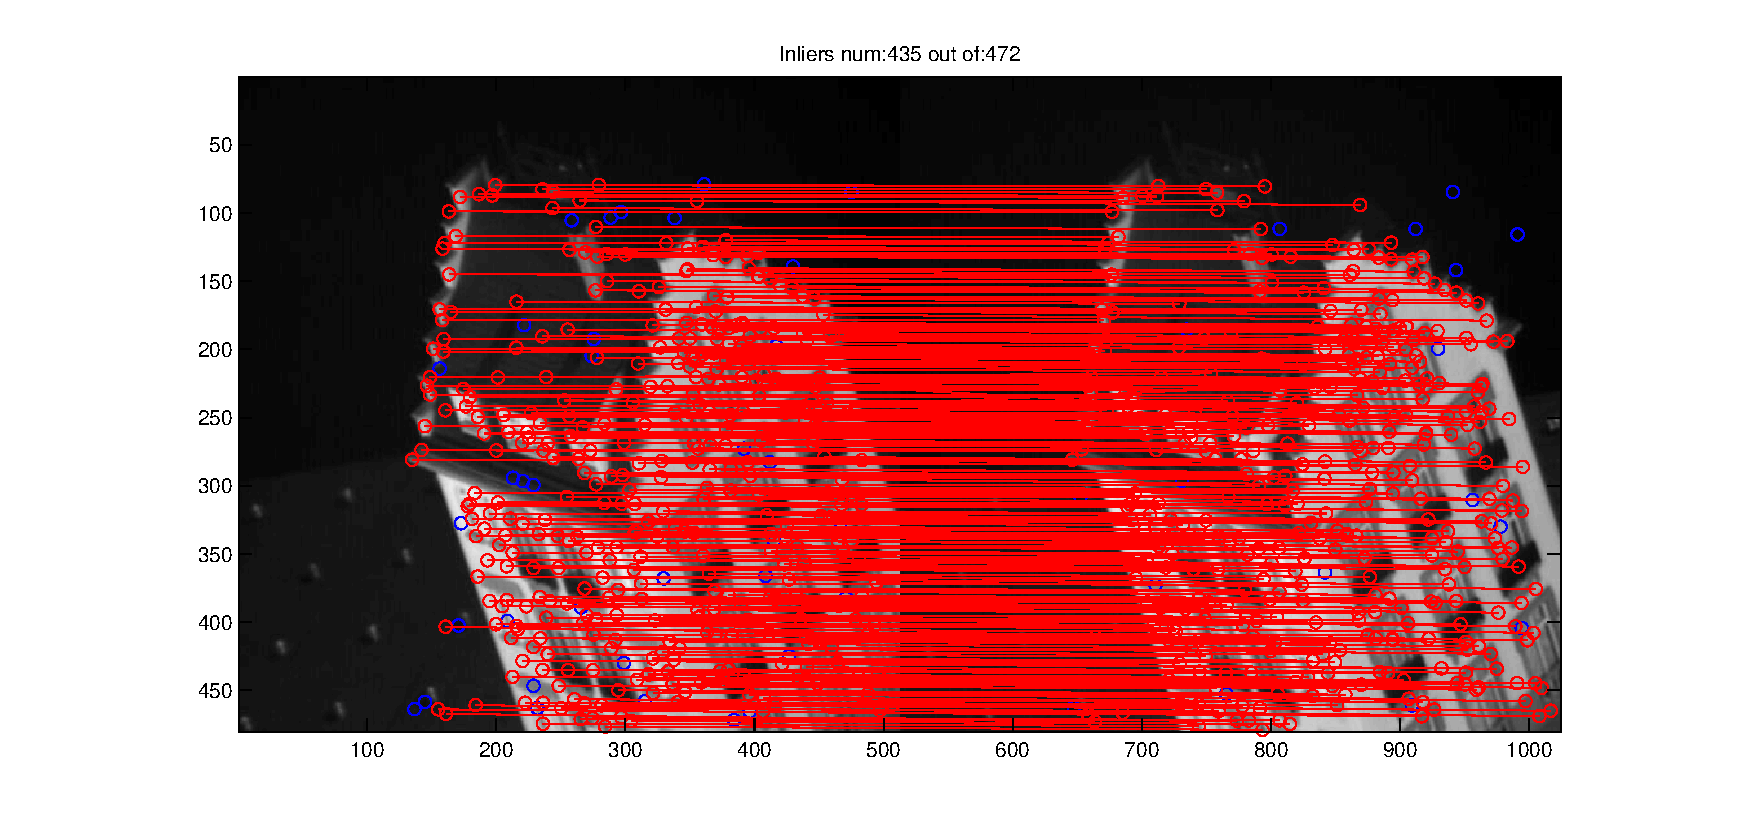
\includegraphics[width=0.55\textwidth]{figures/matchesSimple.eps}\\
    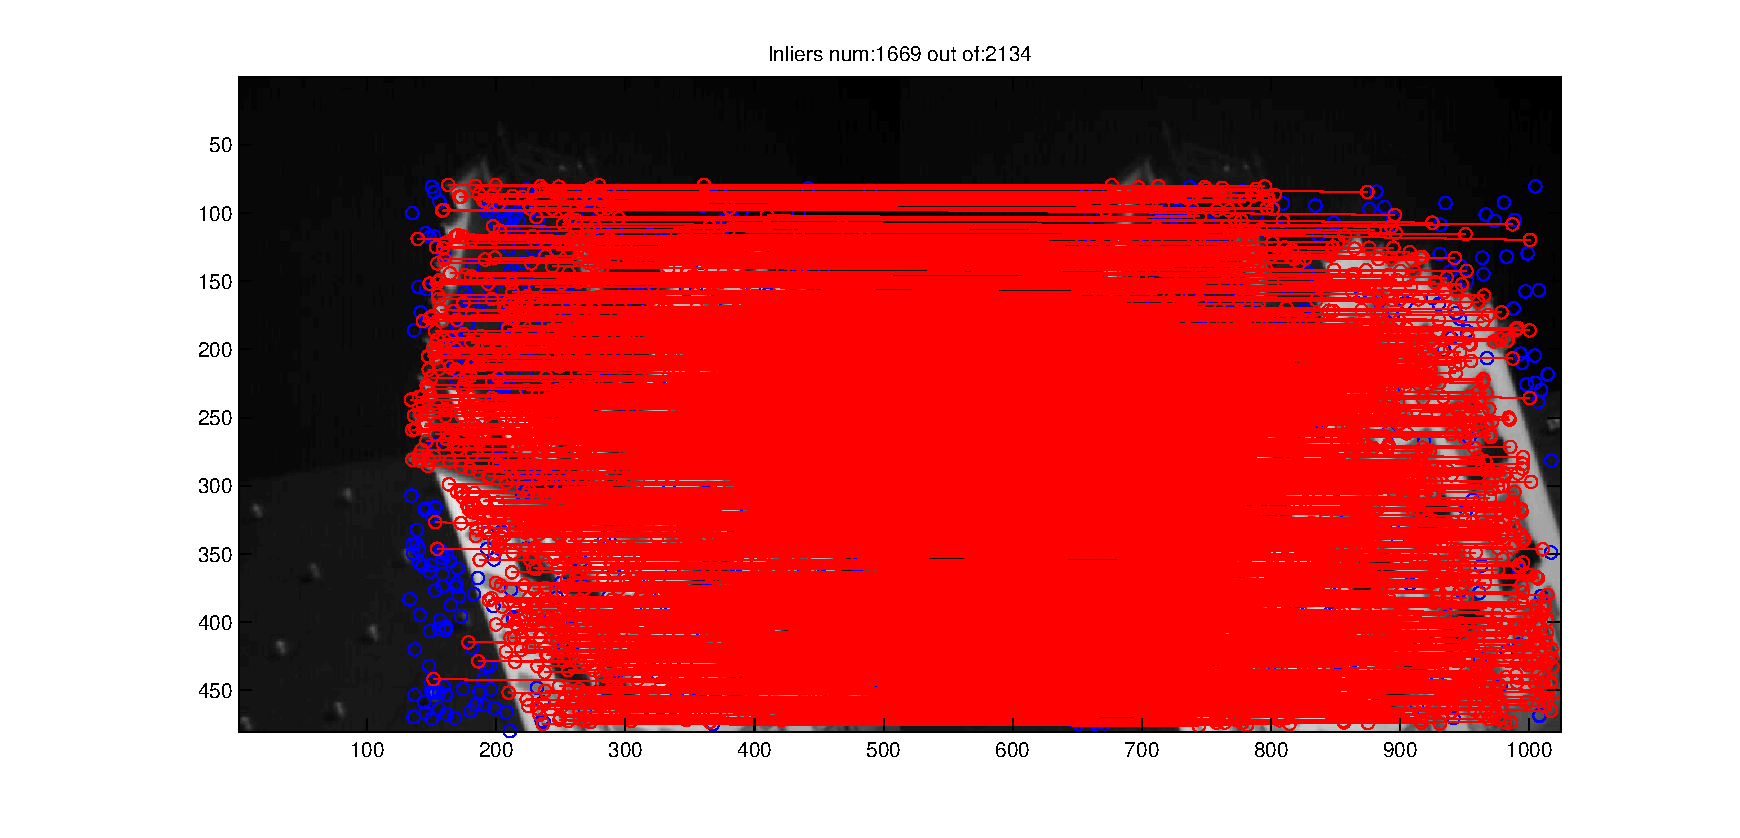
\includegraphics[width=0.55\textwidth]{figures/matchesWithThresh.eps}
    \caption{Above: Feature matches between two consecutive frames without tuned parameters, Below: Feature matches between two consecutive frames with parameter tuning: edgeThresh: 30, Levels: 30.}
    \label{fig:matches}
\end{figure}

The next step is to apply centering to the points, namely subtract the centroid of the feature points (remove translation) according to :

\begin{equation}
\hat{x} = x_{ij} - \frac{1}{n} \sum_{k=1}^{n} x_{ik}
\end{equation}

To estimate the fundamental matrix deriving from the corresponding image points extracted by the SIFT detector the normalized Random Sample Consensus (RANSAC) eight-point algorithm~\cite{eight-point} was implemented. Application of this algorithm leads to a more stable result than the simple eight-point implementation. The steps of the algorithm are:

\begin{enumerate}[1]
  \item Pick 8 random matches from the list of the corresponding points.
  \item Construct a matrix A from the matches and get the transformation matrix from the last column of V of the Singular Value Decomposition of A.
  \item Count the number of inliers (points that agree with the transformation matrix) by computing the Sampson distance (if distance is smaller than a certain threshold then we consider the point as an inlier). By experimenting with different threshold values, we concluded to 0.5 being the most efficient.
  \item Repeat steps 1 to 3 until the majority of the points are inliers.
\end{enumerate}


\subsection{Chaining}
The last step is to construct the Point View Matrix which contains normalized point coordinates (inliers). An $m \times n$ matrix is initialized, where m is the number of frames and n is the total number of feature points. For every point (column) a $1$ is added to the matrix's cell if this feature point is present in frame (row) n, else it remains $0$.

\subsection{Discussion}
In fact, it is not always the case that many points will be present in all frames due to the fact that the frames may have considerably large difference in view among them. In figure~\ref{fig:pointMatching} the feature point view matrices for the house and teddy-bear datasets are illustrated. We can see that the teddy-bear dataset produces a vastly more sparse point view matrix compared to the one the house dataset produces. In particular, no points are consistent through the whole teddy bear frame set. These point view matrices will be used in the $2^{nd}$ part of the SFM implementation, in order to build a 3D structure of these two objects.

\begin{figure}[ht!]
  \centering
    \includegraphics[width=0.50\textwidth]{figures/pvmList.eps}\\
    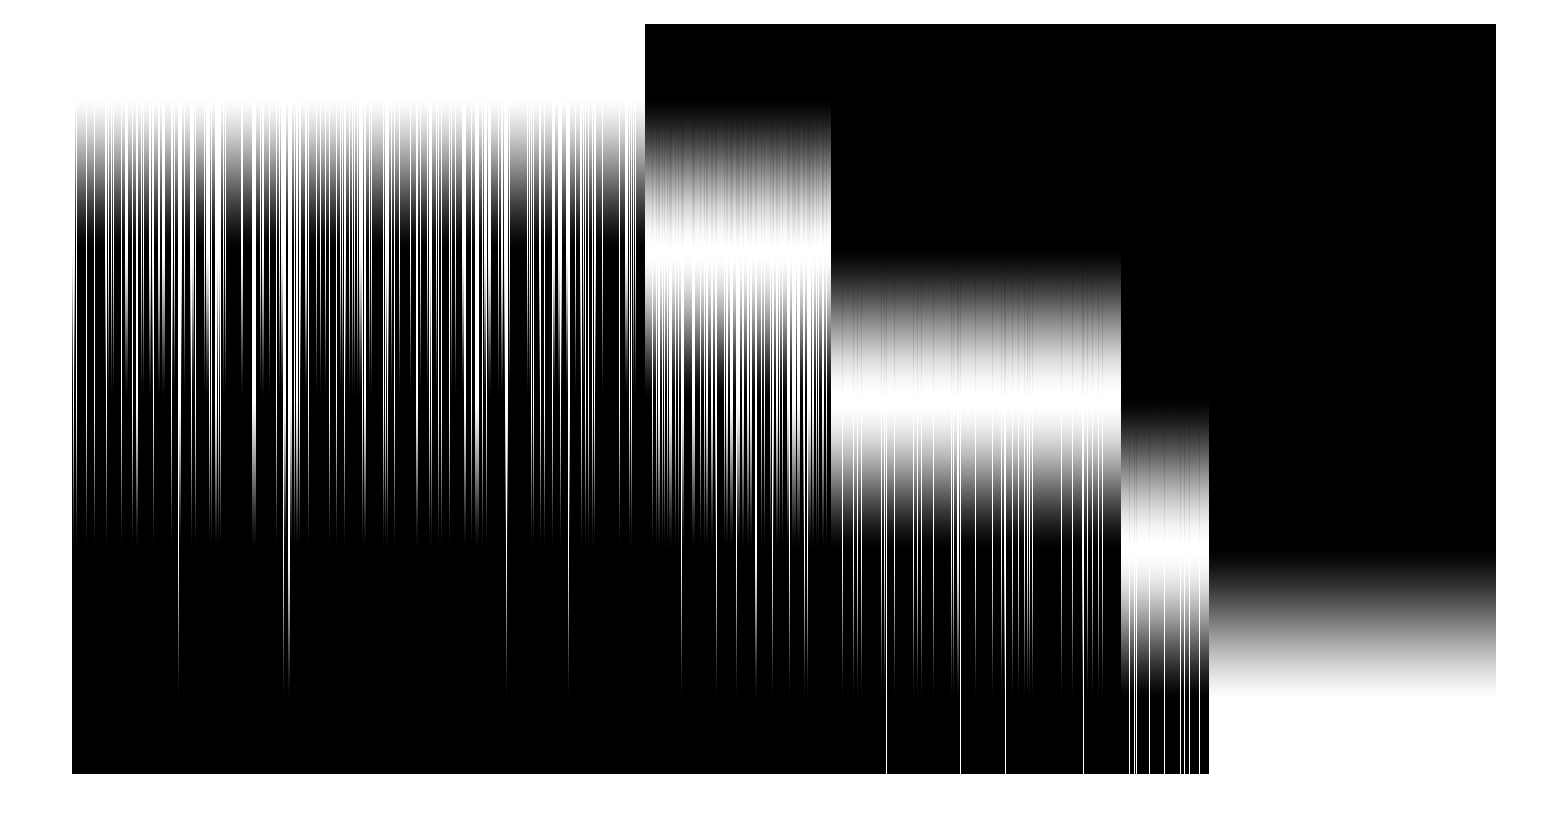
\includegraphics[width=0.50\textwidth]{figures/teddypvm.png}
    \caption{Point view matrix sequences, Horizontal axis denotes detected feature points, vertical axis are the frames. Lines starting from the top going to the bottom of the picture represent points detected in consecutive frames. From top to bottom: a) house dataset, b) teddybear dataset. Note that these Point View matrices result from 3-frame skipping (see 4.3)}
    \label{fig:pointMatching}
\end{figure}

